%%\documentclass[a4paper, 12pt]{scrreprt}

\documentclass[a4paper, 12pt]{scrartcl}
%usepackage[german]{babel}
\usepackage{microtype}
%\usepackage{amsmath}
%usepackage{color}
\usepackage[utf8]{inputenc}
\usepackage[T1]{fontenc}
\usepackage{wrapfig}
\usepackage{lipsum}% Dummy-Text
\usepackage{multicol}
\usepackage{alltt}
%%%%%%%%%%%%bis hierhin alle nötigen userpackage
\usepackage{tabularx}
\usepackage[utf8]{inputenc}
\usepackage{amsmath}
\usepackage{amsfonts}
\usepackage{amssymb}

%\usepackage{wrapfig}
\usepackage[ngerman]{babel}
\usepackage[left=25mm,top=25mm,right=25mm,bottom=25mm]{geometry}
%\usepackage{floatrow}
\setlength{\parindent}{0em}
\usepackage[font=footnotesize,labelfont=bf]{caption}
\numberwithin{figure}{section}
\numberwithin{table}{section}
\usepackage{subcaption}
\usepackage{float}
\usepackage{url}
%\usepackage{fancyhdr}
\usepackage{array}
\usepackage{geometry}
%\usepackage[nottoc,numbib]{tocbibind}
\usepackage[pdfpagelabels=true]{hyperref}
\usepackage[font=footnotesize,labelfont=bf]{caption}
\usepackage[T1]{fontenc}
\usepackage {palatino}
%\usepackage[numbers,super]{natbib}
%\usepackage{textcomp}
\usepackage[version=4]{mhchem}
\usepackage{subcaption}
\captionsetup{format=plain}
\usepackage[nomessages]{fp}
\usepackage{siunitx}
\sisetup{exponent-product = \cdot, output-product = \cdot}
\usepackage{hyperref}
\usepackage{longtable}
\newcolumntype{L}[1]{>{\raggedright\arraybackslash}p{#1}} % linksbündig mit Breitenangabe
\newcolumntype{C}[1]{>{\centering\arraybackslash}p{#1}} % zentriert mit Breitenangabe
\newcolumntype{R}[1]{>{\raggedleft\arraybackslash}p{#1}} % rechtsbündig mit Breitenangabe
\usepackage{booktabs}
\renewcommand*{\doublerulesep}{1ex}
\usepackage{graphicx}


\usepackage[backend=bibtex, style=chem-angew, backref=none, backrefstyle=all+]{biblatex}
\bibliography{Literatur.bib}
\defbibheading{head}{\section{Literatur}\label{sec:Lit}} 
\let\cite=\supercite
%\begin{document}
\section{Durchführung}
Bei einem Aussendruck von \textbf{Druck} bar wurde bei einer Temperatur von 26 \textdegree C die zeitliche Abnahme des Volumen von Isopentan aufgrund von Gasdiffusion  gemessen. Es wurde ein Stefan-Rohr genutzt. 


\begin{figure}[H]

\centering
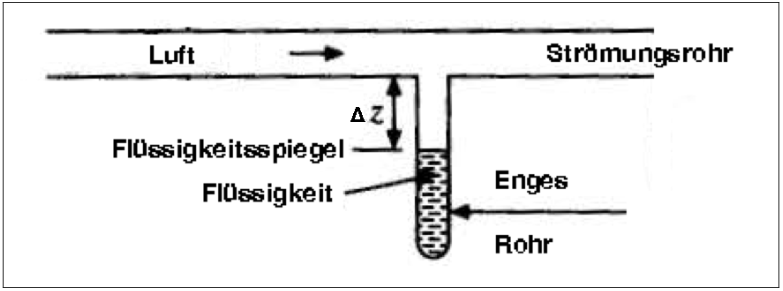
\includegraphics[width=0.8\linewidth]{stefanrohr.png}
\caption{Aus dem Praktikumsskript übernommene Skizze eines Stefan-Rohr. Als Flüssigkeit wurde Isopentan verwendet. Das Volumen sinkt durch Verdampfung kontinuierlich. Dies macht sich darin bemerkbar, das der Abstand z sich ständig vergrößert.}
\end{figure}

Zur Erzeugung des Luftstroms im Strömungsrohr wurde die Auslasseite einer Membranpumpe verwendet. Das Strömungsrohr wurde in eine Silikonöl getaucht und anhand der  Balsengeschwindigkeit von ca zwei Blasen pro Sekunde die Strömungsgeschwindigkeit eingestellt. Das Volumen des Isopentan wurde mittels einer an dem engen Rohr gegebener Skala mittels einer Lupe alle 5 Minuten abgelesen. Insgesamt wurde über \textbf{Zeit} Minuten \textbf{Anzahl} Messwerte aufgenommen.
%\end{document}
